\let\lesson\undefined
\newcommand{\lesson}{\phantomlesson{Bài 16: Công suất. Hiệu suất.}}
\chapter[Hiệu suất]{Hiệu suất}
\setcounter{section}{0}
\section{Lý thuyết}
\subsection{Năng lượng có ích, năng lượng toàn phần}
\begin{minipage}{0.6\textwidth}
	Trong xe ô tô, năng lượng cung cấp cho xe (năng lượng toàn phần) chính là năng lượng hóa học được tạo ra từ việc đốt nhiên liệu. Một phần năng lượng toàn phần được chuyển thành cơ năng (năng lượng có ích) làm xe chuyển động, phần còn lại là năng lượng thất thoát dưới nhiều dạng khác nhau gọi là năng lượng hao phí.
\end{minipage}
\begin{minipage}{0.4\textwidth}
	\begin{center}
		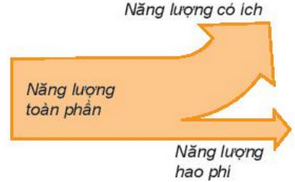
\includegraphics[scale=0.8]{../figs/G10-022-1}
	\end{center}
\end{minipage}

\subsection{Khái niệm hiệu suất}
Gọi công suất toàn phần của động cơ là $\calP$, công suất có ích là $\calP'$.

Hiệu suất của động cơ $H$ là tỉ số giữa công suất có ích và công suất toàn phần của động cơ, đặc trưng cho hiệu quả làm việc của động cơ.
$$H=\dfrac{\calP'}{\calP} \cdot 100\%$$
hoặc hiệu suất cũng có thể tính theo tỉ lệ giữa năng lượng có ích ($W_\text i$) và năng lượng toàn phần ($W_\text{tp}$):
$$H=\dfrac{W_\text{i}}{W_\text{tp}} \cdot 100\%$$

Ví dụ, hiệu suất của động cơ nhiệt được viết dưới dạng:
$$H=\dfrac{A}{Q} \cdot 100\%$$
Trong đó, $A$ là công cơ học mà động cơ thực hiện được, $Q$ là nhiệt lượng mà động cơ nhận được từ nhiên liệu bị đốt cháy.

\textit{Lưu ý:} Hiệu suất của động cơ luôn nhỏ hơn 1, vì không có một máy móc nào hoạt động mà không có sự mất mát năng lượng do ma sát, nhiệt và các dạng năng lượng hao phí khác.

\manatip{
	Để xác định đúng năng lượng có ích và năng lượng hao phí, cần phải hiểu rõ chức năng của thiết bị. Năng lượng phục vụ chức năng của thiết bị là năng lượng có ích. 
	
	Ví dụ như: 
	\begin{itemize}
		\item Ô tô được chế tạo để phục vụ việc di chuyển. Do đó lượng năng lượng chuyển thành động năng là năng lượng có ích, còn những dạng năng lượng khác (làm các bộ phận nóng lên, bị bào mòn,... là năng lượng hao phí).
		\item Quạt máy được chế tạo để xoay tạo ra gió, nên phần năng lượng được chuyển thành động năng quay của quạt là năng lượng có ích, còn năng lượng làm quạt nóng lên là năng lượng hao phí. 
		\item Bếp điện được chế tạo để đun nóng vật khác, nên lượng năng lượng được chuyển thành nhiệt năng của mặt bếp là năng lượng có ích, còn năng lượng làm nóng các bộ phận khác của bếp là năng lượng hao phí. 
	\end{itemize}
}
\section{Mục tiêu bài học - Ví dụ minh họa}
\begin{dang}{Nêu được khái niệm năng lượng có ích và năng lượng hao phí.\\ Suy ra công thức và khái niệm hiệu suất}
	
	\viduii{2}{
		Một động cơ ô tô có hiệu suất $25\%$, thông số này có nghĩa là gì?
	}
	{\begin{center}
			\textbf{Hướng dẫn giải}
		\end{center}
		
		Nói động cơ ô tô có hiệu suất $25\%$ có nghĩa là $25\%$ năng lượng hóa học trong xăng (dầu) được chuyển hóa thành động năng của ô tô, gọi là năng lượng có ích $A_\text{i}$. Phần $75\%$ năng lượng còn lại gọi là năng lượng hao phí $A_\text{hp}$.
		
		\begin{center}
			\textbf{Câu hỏi tương tự}
		\end{center}
		
		Hiệu suất của nhà máy điện dùng năng lượng mặt trời không bằng $1/3 $ hiệu suất của nhà máy nhiệt điện. Tại sao người ta vẫn khuyến khích xây dựng nhà máy điện dùng năng lượng mặt trời?
		
	}
	\viduii{2}{
		Tìm phương án giảm năng lượng hao phí khi sử dụng các thiết bị điện trong gia đình hoặc động cơ ô tô, xe máy.
		
	}
	{\begin{center}
			\textbf{Hướng dẫn giải}
		\end{center}
		
		Các phương án có thể kể đến là
		\begin{itemize}
			\item Thường xuyên vệ sinh thiết bị, tra dầu nhớt để giảm hao phí do tỏa nhiệt, ma sát;
			\item Thường xuyên bảo dưỡng thiết bị và thay thế khi thiết bị đã quá cũ;
			\item Sử dụng thiết bị đúng chức năng và hướng dẫn sử dụng của nhà sản xuất;
			\item Tắt bớt một số chức năng nhất định của thiết bị khi không cần sử dụng.
		\end{itemize}
	}
\end{dang}

\begin{dang}{Vận dụng công thức tính hiệu suất trong một số trường hợp thực tiễn}
	\viduii{2}{Trong mỗi giây, một tấm pin mặt trời có thể hấp thụ $\SI{750}{J}$ năng lượng ánh sáng, nhưng nó chỉ có thể chuyển hóa thành $\SI{120}{J}$ năng lượng điện. Hiệu suất của tấm pin này là bao nhiêu?
	}
	{	\begin{center}
			\textbf{Hướng dẫn giải}
		\end{center}
		
		Hiệu suất của tấm pin là
		$$H=\dfrac{A'}{A} \cdot 100\% = \dfrac{120}{750} \cdot 100\% \approx 16\%$$
		
		
		
	}
	
	
	
	\viduii{3}{Một thùng hàng có khối lượng $\SI{30}{kg}$ được đẩy lên một con dốc cao $\SI{2}{m}$ bằng một động cơ băng chuyền. Hiệu suất của động cơ là bao nhiêu? Biết rằng trong cả quá trình vận chuyển, động cơ cần sử dụng năng lượng tổng là $\SI{5000}{J}$. Lấy $g=\SI{9.8}{m/s^2}$.
	}
	{	\begin{center}
			\textbf{Hướng dẫn giải}
		\end{center}
		
		Công có ích khi thực hiện đẩy thùng hàng lên đến đỉnh dốc là
		$$A'=m\cdot g \cdot h$$
		
		Hiệu suất của động cơ băng chuyền trong quá trình vận chuyển này:
		$$H=\dfrac{A'}{A} \cdot 100\%  = \dfrac{30 \cdot \SI{9.8}{} \cdot 2}{\SI{5000}{}} \cdot 100\% = \SI{11.76}{\percent}.$$
		
		\begin{center}
			\textbf{Câu hỏi tương tự}
		\end{center}
		
		Một động cơ đang hoạt động với công suất $\SI{1000}{W}$ đưa $\SI{100}{kg}$ vật liệu lên đều tới độ cao $\SI{16}{m}$ trong $\SI{20}{s}$. Tính hiệu suất của động cơ.
		
		\textbf{Đáp án:} $80\%$.
	}
	
	\viduii{4}{
		Một xe bán tải có khối lượng $\SI{1.5}{}$ tấn, hiệu suất của xe là $18\%$. Tìm số lít xăng cần dùng để xe tăng tốc đều từ trạng thái nghỉ đến tốc độ $\SI{15}{m/s}$. Biết năng lượng chứa trong $\SI{3.8}{\ell}$ xăng là $\SI{1.3e8}{J}$.
	}
	{	\begin{center}
			\textbf{Hướng dẫn giải}
		\end{center}
		
		Áp dụng định lí động năng để xác định công có ích để xe tăng tốc đều từ trạng thái nghỉ đến tốc độ $\SI{15}{m/s}$:
		$$W_\text{đ2} - W_\text{đ1} = A' \Rightarrow A' = \dfrac{1}{2} \cdot \SI{1500}{} \cdot \SI{15}{}^2 = \SI{168750}{J}$$
		
		Áp dụng công thức tính hiệu suất để xác định năng lượng toàn phần do nhiên liệu bị đốt:
		$$H=\dfrac{A'}{A} \cdot 100\% \Rightarrow A=\dfrac{A'}{H} \cdot 100\% = \SI{937500}{J}$$
		
		Số lít xăng cần dùng:
		$$V=\dfrac{\SI{3.8}{} \cdot \SI{937500}{}}{\SI{1.3e8}{}} = \SI{0.027}{\ell}$$
		
		\begin{center}
			\textbf{Câu hỏi tương tự}
		\end{center}
		
		Một ô tô chuyển động thẳng đều với vận tốc $\SI{54}{km/h}$ có thể đi được đoạn đường dài bao nhiêu khi tiêu thụ hết 60 lít xăng? Biết động cơ của ô tô có công suất $\SI{45}{kW}$; hiệu suất $25\%$; với $\SI{1}{kg}$ xăng đốt cháy hoàn toàn tỏa ra nhiệt lượng bằng $\SI{46e6}{J}$ và khối lượng riêng của xăng là $\SI{700}{kg/m^3}$.
		
		\textbf{Đáp án:} $\SI{161}{km}$.
	}
\end{dang}